
\documentclass[border=10pt, 12pt]{standalone}
\usepackage[svgnames]{xcolor}
\usepackage{amsmath}
\usepackage{pgfplots}
\pgfplotsset{compat=newest}
\usepackage[sfdefault]{FiraSans}
\usepackage{FiraMono}
\renewcommand*\familydefault{\sfdefault}
\begin{document}
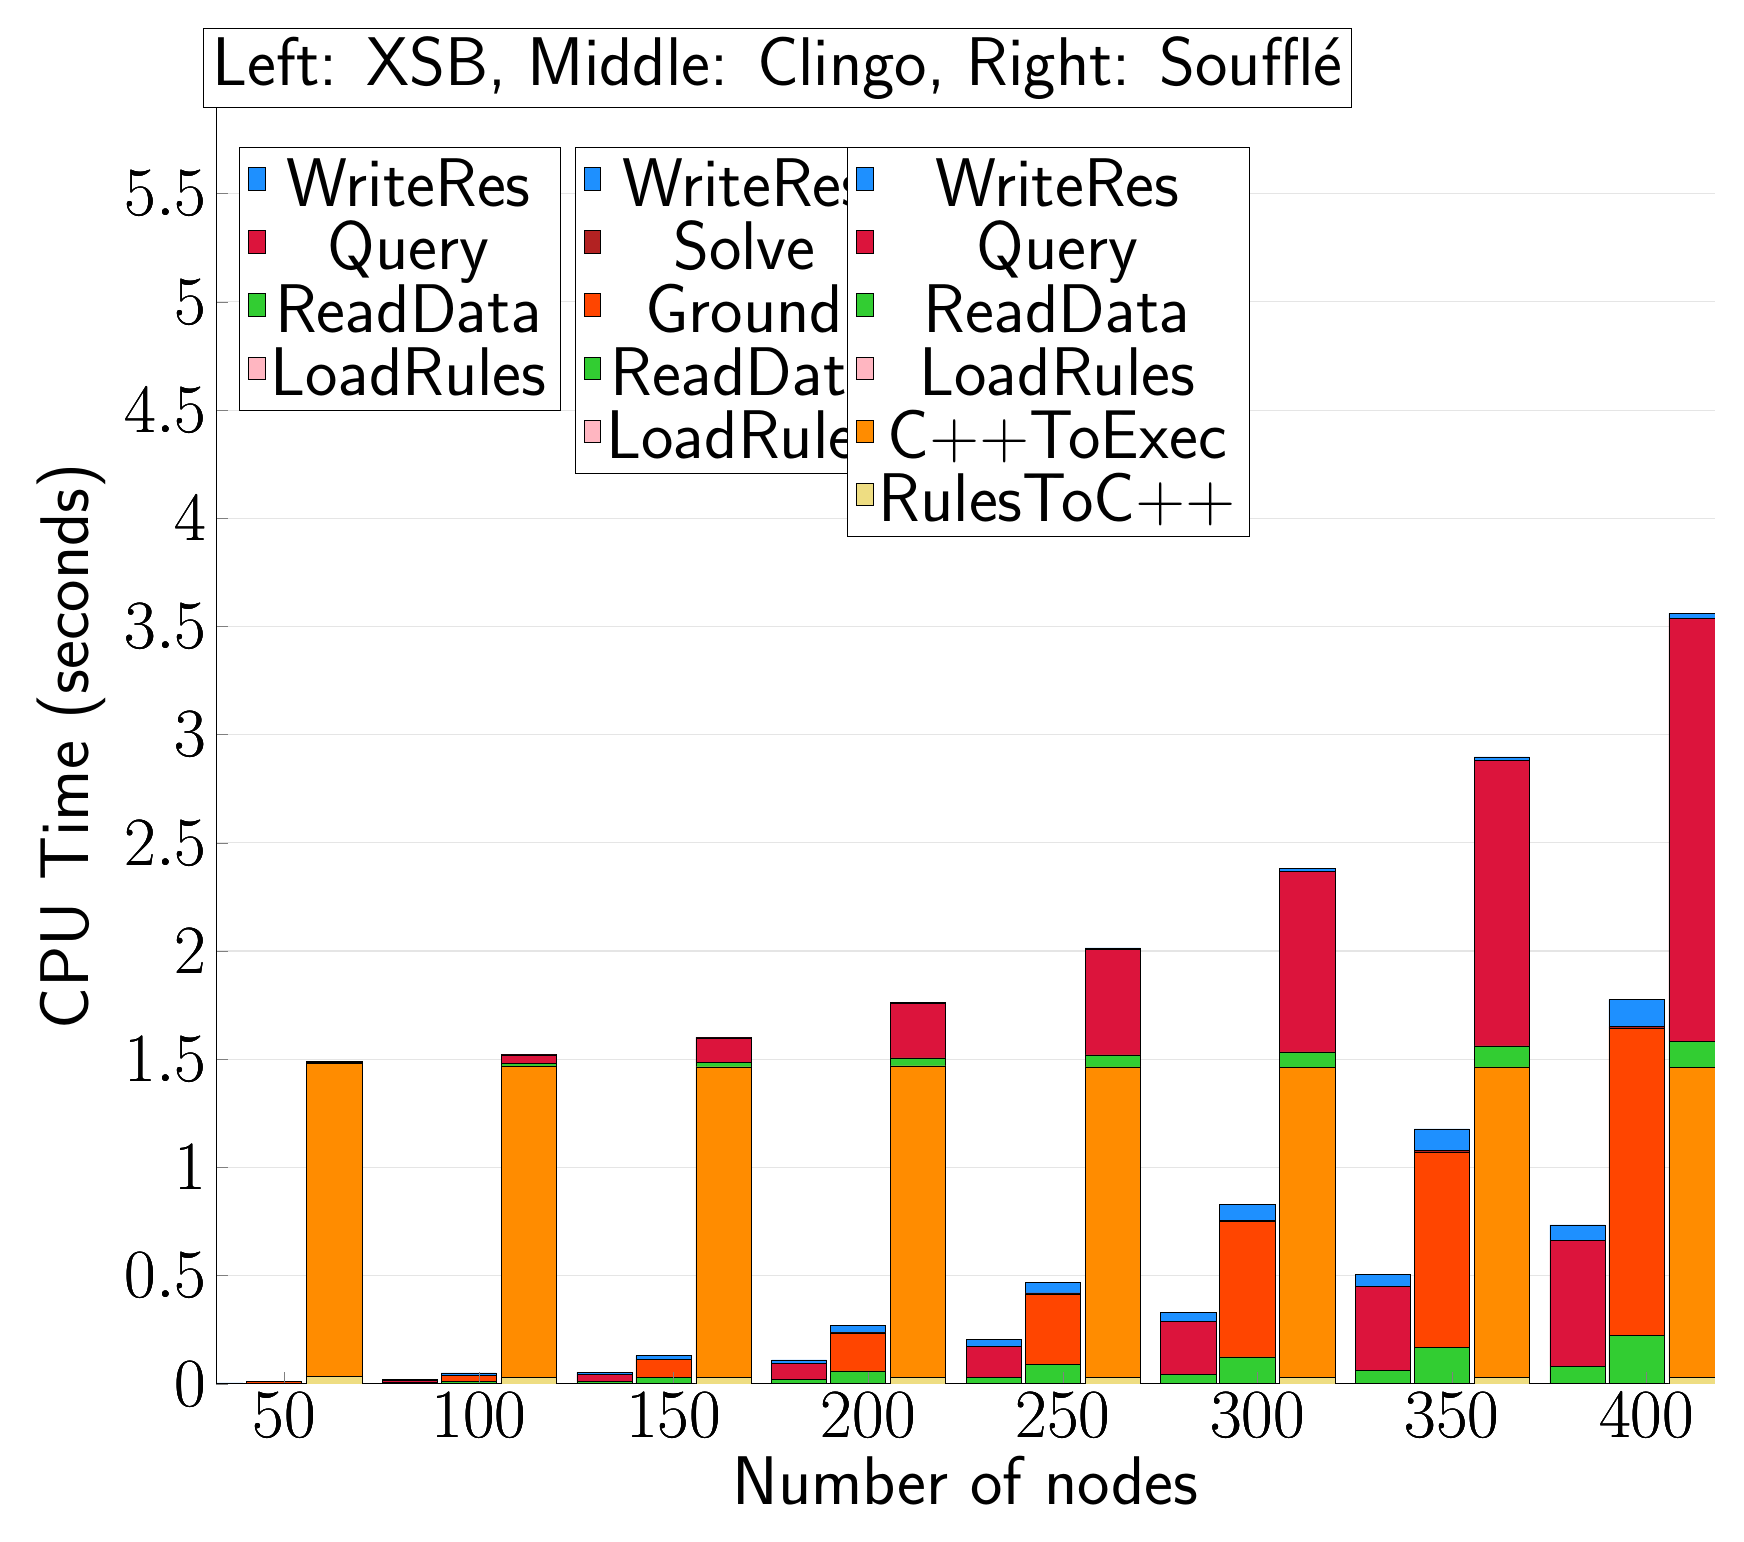
\begin{tikzpicture}
	\begin{axis}[bar shift=-25pt,
			ybar stacked,
			width=1.7\textwidth,
			bar width=0.7cm,
			ymajorgrids, tick align=inside,
			major grid style={draw=gray!20},
			xtick=data,
			ymin=0, ymax=5.893940000000001,
			axis x line*=bottom,
			axis y line*=left,
			enlarge x limits=0.05,
			legend style={
					at={(0.23, 0.97)},
					anchor=north east,
					legend columns=1,
					font=\Huge,
				},
			ylabel={CPU Time (seconds)},
			xlabel={Number of nodes},
			label style={font=\Huge},
			tick label style={font=\Huge},
		]
		\addlegendimage{fill=DodgerBlue, draw=black, line width=0.2pt}
		\addlegendentry{WriteRes}
		\addlegendimage{fill=Crimson, draw=black, line width=0.2pt}
		\addlegendentry{Query}
		\addlegendimage{fill=LimeGreen, draw=black, line width=0.2pt}
		\addlegendentry{ReadData}
		\addlegendimage{fill=LightPink, draw=black, line width=0.2pt}
		\addlegendentry{LoadRules}
		\addplot +[fill=LightPink, draw=black, line width=0.2pt] coordinates {
				(50, 0.0006271)
				(100, 0.0006166000000000004)
				(150, 0.0006108999999999996)
				(200, 0.0006007999999999996)
				(250, 0.0005962999999999998)
				(300, 0.0006098000000000001)
				(350, 0.0006278999999999996)
				(400, 0.0006121)
			};
		\addplot +[fill=LimeGreen, draw=black, line width=0.2pt] coordinates {
				(50, 0.0011819)
				(100, 0.0044548999999999995)
				(150, 0.0102316)
				(200, 0.0185252)
				(250, 0.029668099999999996)
				(300, 0.04331809999999999)
				(350, 0.060356900000000005)
				(400, 0.0799406)
			};
		\addplot +[fill=Crimson, draw=black, line width=0.2pt] coordinates {
				(50, 0.0012682000000000001)
				(100, 0.0094437)
				(150, 0.0312102)
				(200, 0.073782)
				(250, 0.1443604)
				(300, 0.24582600000000002)
				(350, 0.3891722)
				(400, 0.5827848)
			};
		\addplot +[fill=DodgerBlue, draw=black, line width=0.2pt] coordinates {
				(50, 0.0011434)
				(100, 0.004635599999999999)
				(150, 0.0104344)
				(200, 0.017969600000000002)
				(250, 0.029538999999999992)
				(300, 0.04214179999999999)
				(350, 0.0556636)
				(400, 0.07121339999999997)
			};
	\end{axis}

	\begin{axis}[bar shift=-3.7pt,
			ybar stacked,
			width=1.7\textwidth,
			bar width=0.7cm,
			ymajorgrids, tick align=inside,
			major grid style={draw=none},
			xtick=data,
			ymin=0, ymax=5.893940000000001,
			axis x line*=none,
			axis y line*=none,
			enlarge x limits=0.05,
			legend style={
					at={(0.454, 0.97)},
					anchor=north east,
					legend columns=1,
					font=\Huge,
				},
			label style={font=\Huge},
			tick label style={font=\Huge},
		]
		\addlegendimage{fill=DodgerBlue, draw=black, line width=0.2pt}
		\addlegendentry{WriteRes}
		\addlegendimage{fill=FireBrick, draw=black, line width=0.2pt}
		\addlegendentry{Solve}
		\addlegendimage{fill=OrangeRed, draw=black, line width=0.2pt}
		\addlegendentry{Ground}
		\addlegendimage{fill=LimeGreen, draw=black, line width=0.2pt}
		\addlegendentry{ReadData}
		\addlegendimage{fill=LightPink, draw=black, line width=0.2pt}
		\addlegendentry{LoadRules}
		\addplot +[fill=LightPink, draw=black, line width=0.2pt] coordinates {
				(50, 0.0)
				(100, 0.0)
				(150, 0.0)
				(200, 0.0)
				(250, 0.0)
				(300, 0.0)
				(350, 0.0)
				(400, 0.0)
			};
		\addplot +[fill=LimeGreen, draw=black, line width=0.2pt] coordinates {
				(50, 0.0)
				(100, 0.009999999999999997)
				(150, 0.030000000000000006)
				(200, 0.06000000000000001)
				(250, 0.08999999999999998)
				(300, 0.12400000000000003)
				(350, 0.16999999999999998)
				(400, 0.22300000000000003)
			};
		\addplot +[fill=OrangeRed, draw=black, line width=0.2pt] coordinates {
				(50, 0.009999999999999997)
				(100, 0.030000000000000006)
				(150, 0.08199999999999999)
				(200, 0.17499999999999996)
				(250, 0.326)
				(300, 0.6279999999999999)
				(350, 0.9010000000000001)
				(400, 1.418)
			};
		\addplot +[fill=FireBrick, draw=black, line width=0.2pt] coordinates {
				(50, 0.0)
				(100, 0.0)
				(150, 0.0010000000000000009)
				(200, 0.0030000000000000027)
				(250, 0.0040000000000000036)
				(300, 0.0020000000000000018)
				(350, 0.007000000000000006)
				(400, 0.010000000000000009)
			};
		\addplot +[fill=DodgerBlue, draw=black, line width=0.2pt] coordinates {
				(50, 0.0)
				(100, 0.010000000000000009)
				(150, 0.016999999999999994)
				(200, 0.03099999999999999)
				(250, 0.046999999999999986)
				(300, 0.07599999999999997)
				(350, 0.09999999999999987)
				(400, 0.12500000000000006)
			};
	\end{axis}

	\begin{axis}[bar shift=18pt,
			ybar stacked,
			width=1.7\textwidth,
			bar width=0.7cm,
			ymajorgrids, tick align=inside,
			major grid style={draw=none},
			xtick=data,
			ymin=0, ymax=5.893940000000001,
			axis x line*=none,
			axis y line*=none,
			enlarge x limits=0.05,
			legend style={
					at={(0.69, 0.97)},
					anchor=north east,
					legend columns=1,
					font=\Huge,
				},
			label style={font=\Huge},
			tick label style={font=\Huge},
		]
		\addlegendimage{fill=DodgerBlue, draw=black, line width=0.2pt}
		\addlegendentry{WriteRes}
		\addlegendimage{fill=Crimson, draw=black, line width=0.2pt}
		\addlegendentry{Query}
		\addlegendimage{fill=LimeGreen, draw=black, line width=0.2pt}
		\addlegendentry{ReadData}
		\addlegendimage{fill=LightPink, draw=black, line width=0.2pt}
		\addlegendentry{LoadRules}
		\addlegendimage{fill=DarkOrange, draw=black, line width=0.2pt}
		\addlegendentry{C++ToExec}
		\addlegendimage{fill=LightGoldenrod, draw=black, line width=0.2pt}
		\addlegendentry{RulesToC++}
		\addplot +[fill=LightGoldenrod, draw=black, line width=0.2pt] coordinates {
				(50, 0.033)
				(100, 0.030000000000000006)
				(150, 0.030000000000000006)
				(200, 0.030000000000000006)
				(250, 0.030000000000000006)
				(300, 0.030000000000000006)
				(350, 0.030000000000000006)
				(400, 0.030000000000000006)
			};
		\addplot +[fill=DarkOrange, draw=black, line width=0.2pt] coordinates {
				(50, 1.448)
				(100, 1.4389999999999998)
				(150, 1.4349999999999998)
				(200, 1.4389999999999996)
				(250, 1.4349999999999998)
				(300, 1.4329999999999998)
				(350, 1.4349999999999996)
				(400, 1.4329999999999998)
			};
		\addplot +[fill=LightPink, draw=black, line width=0.2pt] coordinates {
				(50, 0.0)
				(100, 0.0)
				(150, 2.16e-05)
				(200, 2.03e-05)
				(250, 0.0)
				(300, 1.0399999999999999e-05)
				(350, 0.0)
				(400, 1.0399999999999999e-05)
			};
		\addplot +[fill=LimeGreen, draw=black, line width=0.2pt] coordinates {
				(50, 0.0026730000000000005)
				(100, 0.0105891)
				(150, 0.0219944)
				(200, 0.0375268)
				(250, 0.054893199999999996)
				(300, 0.07124079999999999)
				(350, 0.0969935)
				(400, 0.12030420000000001)
			};
		\addplot +[fill=Crimson, draw=black, line width=0.2pt] coordinates {
				(50, 0.006233)
				(100, 0.040098600000000005)
				(150, 0.1114307)
				(200, 0.2520518)
				(250, 0.4860805)
				(300, 0.8343223999999999)
				(350, 1.3182200000000002)
				(400, 1.954606)
			};
		\addplot +[fill=DodgerBlue, draw=black, line width=0.2pt] coordinates {
				(50, 0.0006344)
				(100, 0.0015956999999999998)
				(150, 0.0032696999999999995)
				(200, 0.0057109000000000005)
				(250, 0.0088309)
				(300, 0.0125509)
				(350, 0.0170472)
				(400, 0.022152500000000002)
			};
	\end{axis}


	\node[anchor=south, draw, fill=white] at (rel axis cs:0.42,1) {\Huge Left: XSB, Middle: Clingo, Right: Soufflé};
\end{tikzpicture}
\end{document}
